%!TEX root = ../template.tex

\chapter{Validation and Experimental Evaluation}
\label{cha:validation_experimental_Evaluation}

This chapter presents, analyses and discusses the work performed to obtain relevant evaluation criteria measured from the complete system deployed on a cloud environment, in order to validate the implemented prototype.

Section \ref{sec:testbench_environment} details how the system is deployed, explains the different configurations that that system adopts in order to present relevant data to compare.

In section \ref{sec:revelant_evaluation_criteria} explains which metrics will be evaluated for each different testbench scenario. Sections \ref{sec:performance_evaluation_redis_benchmark_tool} through \ref{sec:complementary_measurements} presents the actual metrics taken from the performance and load testing tools and compares the different system configurations with secure and vulnerable storage instances.

The last section, section \ref{sec:summary_and_findings} contains a summary of all the finding and some considerations that can be taken from the presented metrics.

\section{Testbench Environments}
\label{sec:testbench_environment}

The prototype was evaluated in multiple different system configurations to achieve a complete coverage of all the proposed solutions and all the relevant metrics. 

The first test is a representative test of the overhead introduced not only of additional security features like \gls{TLS} and authentication but also the \gls{SGX} hardware isolation. It will run the \textit{redis-benchmark} tool both externally to the server and internally directly against a single standalone Redis instance bypassing the proxy server. Secondly, and more real-life tests, test are run against the proxy exposed \gls{API} and a single standalone Redis instance composes the storage server. Then, the same tests were run in the same environment but with a cluster of Redis instances composing the backend storage. The fourth testbench measures the performance of homomorphic operations on a standalone Redis instance running on unprotected memory, and finally, it is presented the metrics for the two different attestation operations on Redis instances deployed on protected memory and isolated through \gls{SGX}.

All tests performed on the secure prototype are measured several times, averaged and compared with a standard Redis deployment so the overhead of extra security can be evaluated and analysed. 

\section{Relevant Evaluation Criteria}
\label{sec:revelant_evaluation_criteria}

The tests measure several different relevant metrics that can be compared with each other: 

\begin{itemize}
  \item \textbf{Latency} - Measured in milliseconds (ms) and evaluate the round trip response times between the client and the server.
  \item \textbf{Throughput} - Measured in operations per seconds (ops/s) indicates the number of operations the client performed in one second.
  \item \textbf{Startup Times} - Measured in seconds (s) is particularly important to analyse the \gls{SGX} attestation that happens at startup
  \item \textbf{Memory Consumption} - Extracted in megabytes (MB) or a percentage, and measured alongside the tests.
  \item \textbf{\gls{CPU} Consumption} - Extracted in megabytes in a percentage, and also measured alongside the tests.
\end{itemize}

\section{Performance evaluation for Redis-Benchmark tool}
\label{sec:performance_evaluation_redis_benchmark_tool}

The first testbench is performed directly against the Redis server bypassing the proxy. This test was performed with the \textbf{redis-benchmark} \footnote{Since Redis TLS is fairly new, the latest official redis-benchmark realest does not support TLS test. The redis benchmark used comes from the Redis unstable branch (commit a0576bd), but after some analyses it appears to be a final version of the tool. All benchmarks tests used the same version} tool and evaluates the latency and throughput of a basic set of operations - \textit{ping}, \textit{set}, and \textit{get}. It compares three different deployed Redis configurations, where the first one is completely default and open, the second one implements the built-in security features of Redis such as \gls{TLS} and authentication and the third one, not only using the built-in features but also running isolated inside an \gls{SGX} enclave.

Figure \ref{fig:redis_benchmark_external_metrics} presents the latency and throughput results over one hundred thousand requests with 50 multiple concurrent clients and a 3 byte payload when running the benchmark tool on a Macbook Pro 2018 2,3 GHz Quad-Core Intel Core i5 and internet connection averaging the 500Mb/s download and 100Mb/s upload.

\begin{figure}[htbp]
  \centering
  \subcaptionbox{Redis Latency Result\label{fig:redis_latency_external}}%
    {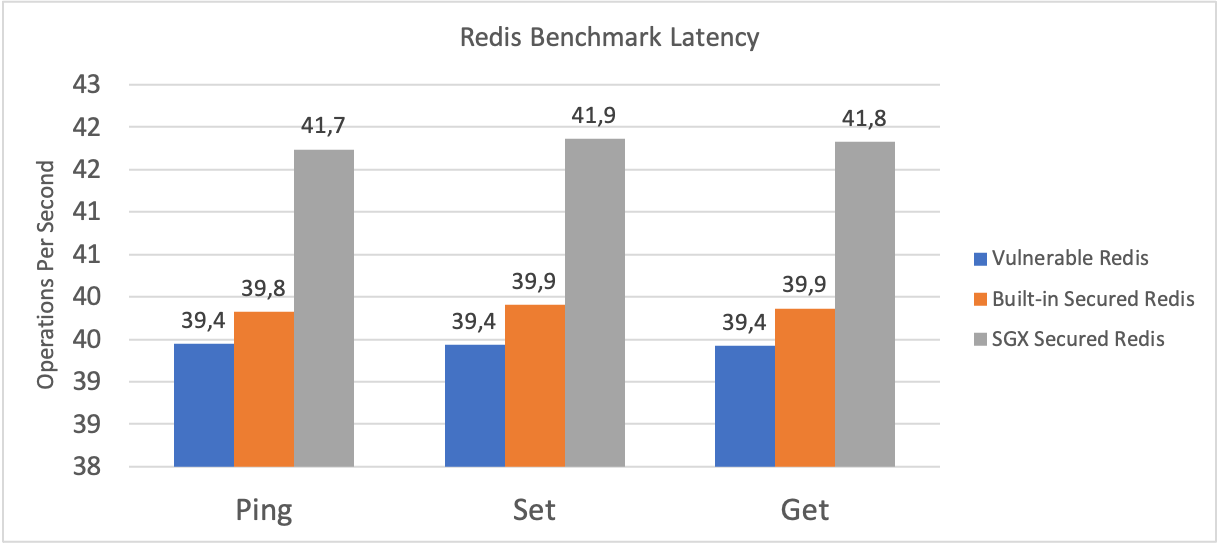
\includegraphics[width=0.5\linewidth]{redis_latency_external}}%
    %\hspace{1em}
  \subcaptionbox{Redis Throughput Result\label{fig:redis_throughput_external_2}}%
    {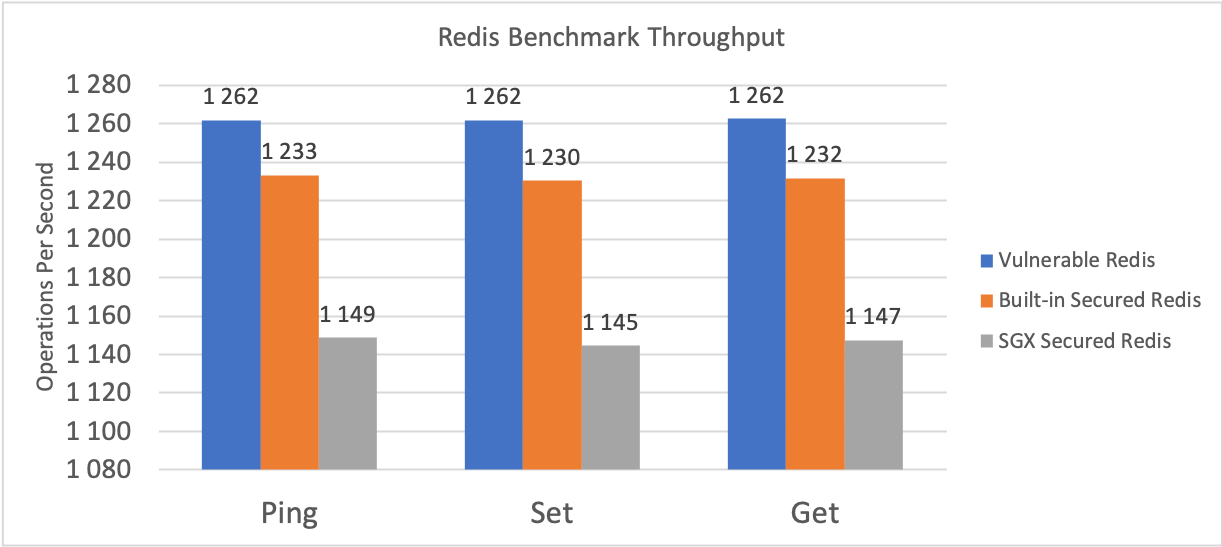
\includegraphics[width=0.5\linewidth]{redis_throughput_external_2}}%
  \caption{Redis Benchmark External Client Metrics}
  \label{fig:redis_benchmark_external_metrics}
\end{figure}

The results show a performance drop for each additional security layers added to the instance deployment. The \gls{SGX} deployed instance showed the biggest overhead on performance, around x\%, both latency and throughput, however, due to the added security, this is an expected result.

Figure \ref{fig:redis_benchmark_internal_metrics} shows the results of the same tests but instead of running the benchmark tool on a separate machine, it runs it on the same host where the server is deployed, therefore eliminating the network overhead.

\begin{figure}[htbp]
  \centering
  \subcaptionbox{Redis Latency Internal\label{fig:redis_latency_internal}}%
    {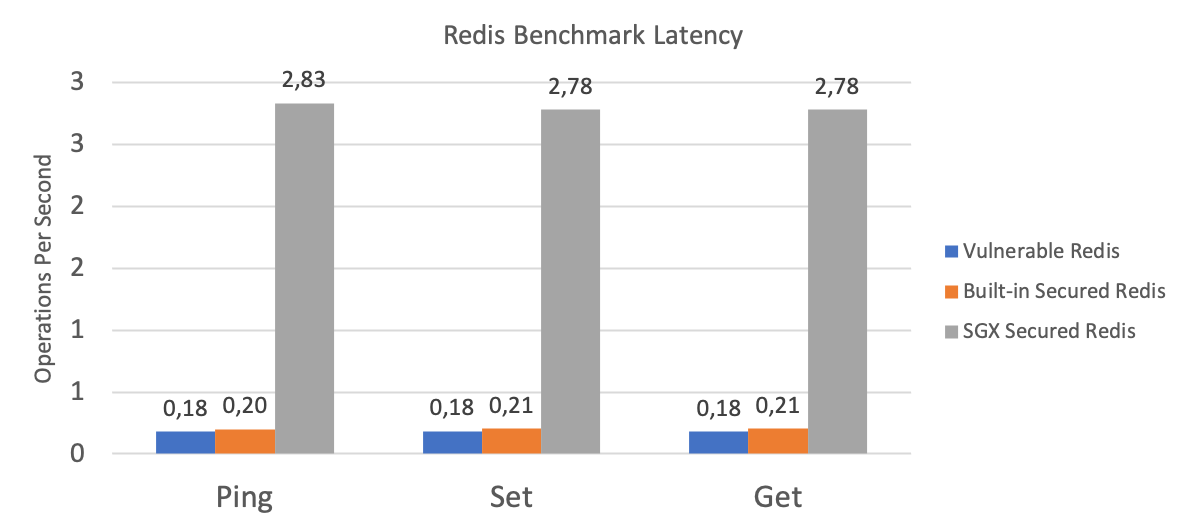
\includegraphics[width=0.5\linewidth]{redis_latency_internal}}%
    %\hspace{1em}
  \subcaptionbox{Redis Throughput Internal\label{fig:redis_throughput_internal}}%
    {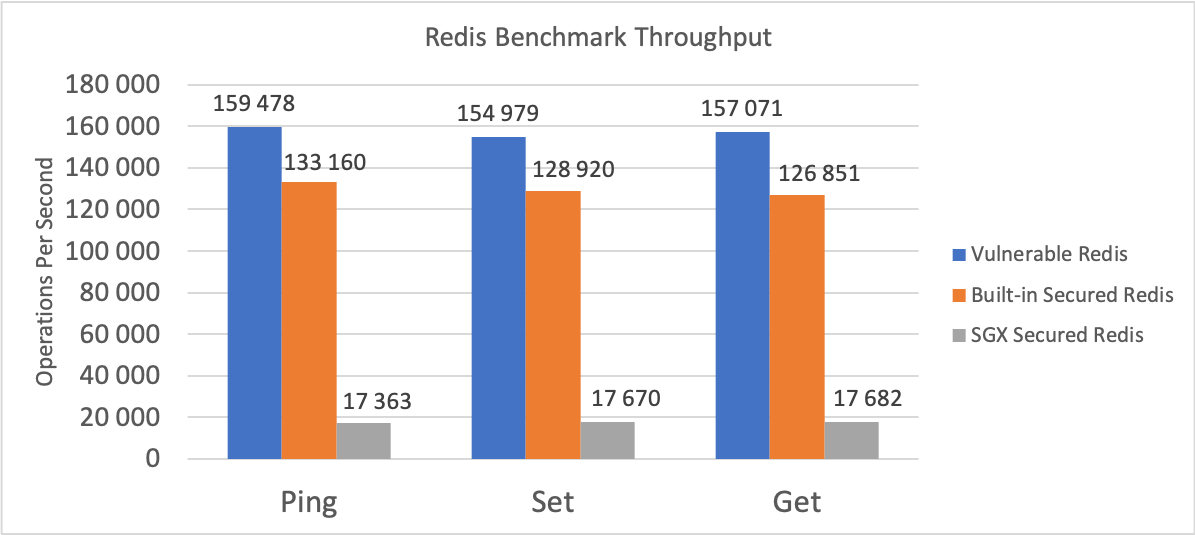
\includegraphics[width=0.5\linewidth]{redis_throughput_internal}}%
  \caption{Redis Benchmark Internal Client Metrics}
  \label{fig:redis_benchmark_internal_metrics}
\end{figure}

The results corroborate the initial tests but the differences between security levels are much more visible. The main objective of this comparison is to point out that the network jitter and latency overhead will affect the performance results going forward to the next tests.

\section{Performance evaluation for Standalone Redis}
\label{sec:performance_evaluation_standalone_redis}

\section{Performance evaluation for Cluster Redis}
\label{sec:performance_evaluation_cluster_redis}

\section{Performance evaluation for Homomorphic Operations}
\label{sec:performance_evaluation_homomorphic_operations}

\section{Evaluation of the Attestation Protocol}
\label{sec:evaluation_attestation_protocol}

Get startup times with and without CAS, get stack attestation times...

\section{Complementary Measurements}
\label{sec:complementary_measurements}

Memory, CPU, etc instrumentation, workload

\section{ Summary and Findings}
\label{sec:summary_and_findings}

% \section{Performance evaluation for Testbench 1}
% \label{sec:performance_evaluation_testbench_1}

% \subsection{Latency}
% \label{ssec:testbench_1_latency}

% \subsection{Throughput}
% \label{ssec:testbench_1_throughput}

% \section{Performance evaluation for Testbench 2}
% \label{sec:performance_evaluation_testbench_2}

% \subsection{Latency}
% \label{ssec:testbench_2_latency}

% \subsection{Throughput}
% \label{ssec:testbench_2_throughput}

% \section{Evaluation of the Attestation Protocol}
% \label{sec:evaluation_attestation_protocol}

% Get startup times with and without CAS, get stack attestation times...

% \section{Complementary Measurements}
% \label{sec:complementary_measurements}

% Memory, CPU, etc instrumentation, workload

% \section{ Summary and Findings}
% \label{sec:summary_and_findings}
